\documentclass[a4paper, oneside, 11pt, onecolumn]{article}


\usepackage{graphicx}
\usepackage{subfig}
\usepackage[round, comma, sort&compress, longnamesfirst]{natbib} 
\usepackage[left=2cm,top=3cm,right=1.5cm,bottom=2cm,bindingoffset=0.5cm]{geometry}
\usepackage{enumerate}
\usepackage{fancyhdr}
\pagestyle{fancy}
\fancyhead{}
\fancyfoot{}
\fancyfoot[L]{\textit{}}
 \fancyhead[L]{\textit{Clarke et al (20xx)}}
\renewcommand{\headrulewidth}{0.8pt}
\renewcommand{\footrulewidth}{0.8pt}
\setlength\headheight{14pt}
\fancyfoot[RO] {\thepage}
\usepackage{authblk}
%%%%%%%%%%%%

\begin{document}

\title{Supplementary Materials}

\author{A. D. F. Clarke\thanks{a.clarke@essex.ac.uk}}
 \affil{School of Psychology, University of Essex, UK}



\maketitle

\begin{abstract}

\end{abstract}

%%%%%%%%%%%%%%%%%%%%%%%%%%%%
\section{Participants}
%%%%%%%%%%%%%%%%%%%%%%%%%%%%

Data was collected from 64 participants as originally planned. Four of these participants did not complete all parts of the experiment (either declining to participate in the second session, or could not be calibrated with the eye tracker), so four new participants were recruited to bring the total back up to 64. 

\subsection{Split-Half}

Accuracy data from all participants is shown in Figure \ref{fig:splithalf_acc_all}. From this we can see that there are a number of outliers: 4, 21, 33, 56, and 58. These participants, in at least one session, either missed the majority of easy targets, or responded with false positives on the majority of target absent trials. After removing these participants, the lowest accuracy in either session was $84.6\%$ for the easy targets, and $76.9\%$ for target absent trials. This leaves us with 59 participants for the split-half paradigm. 

\begin{figure}
\centering
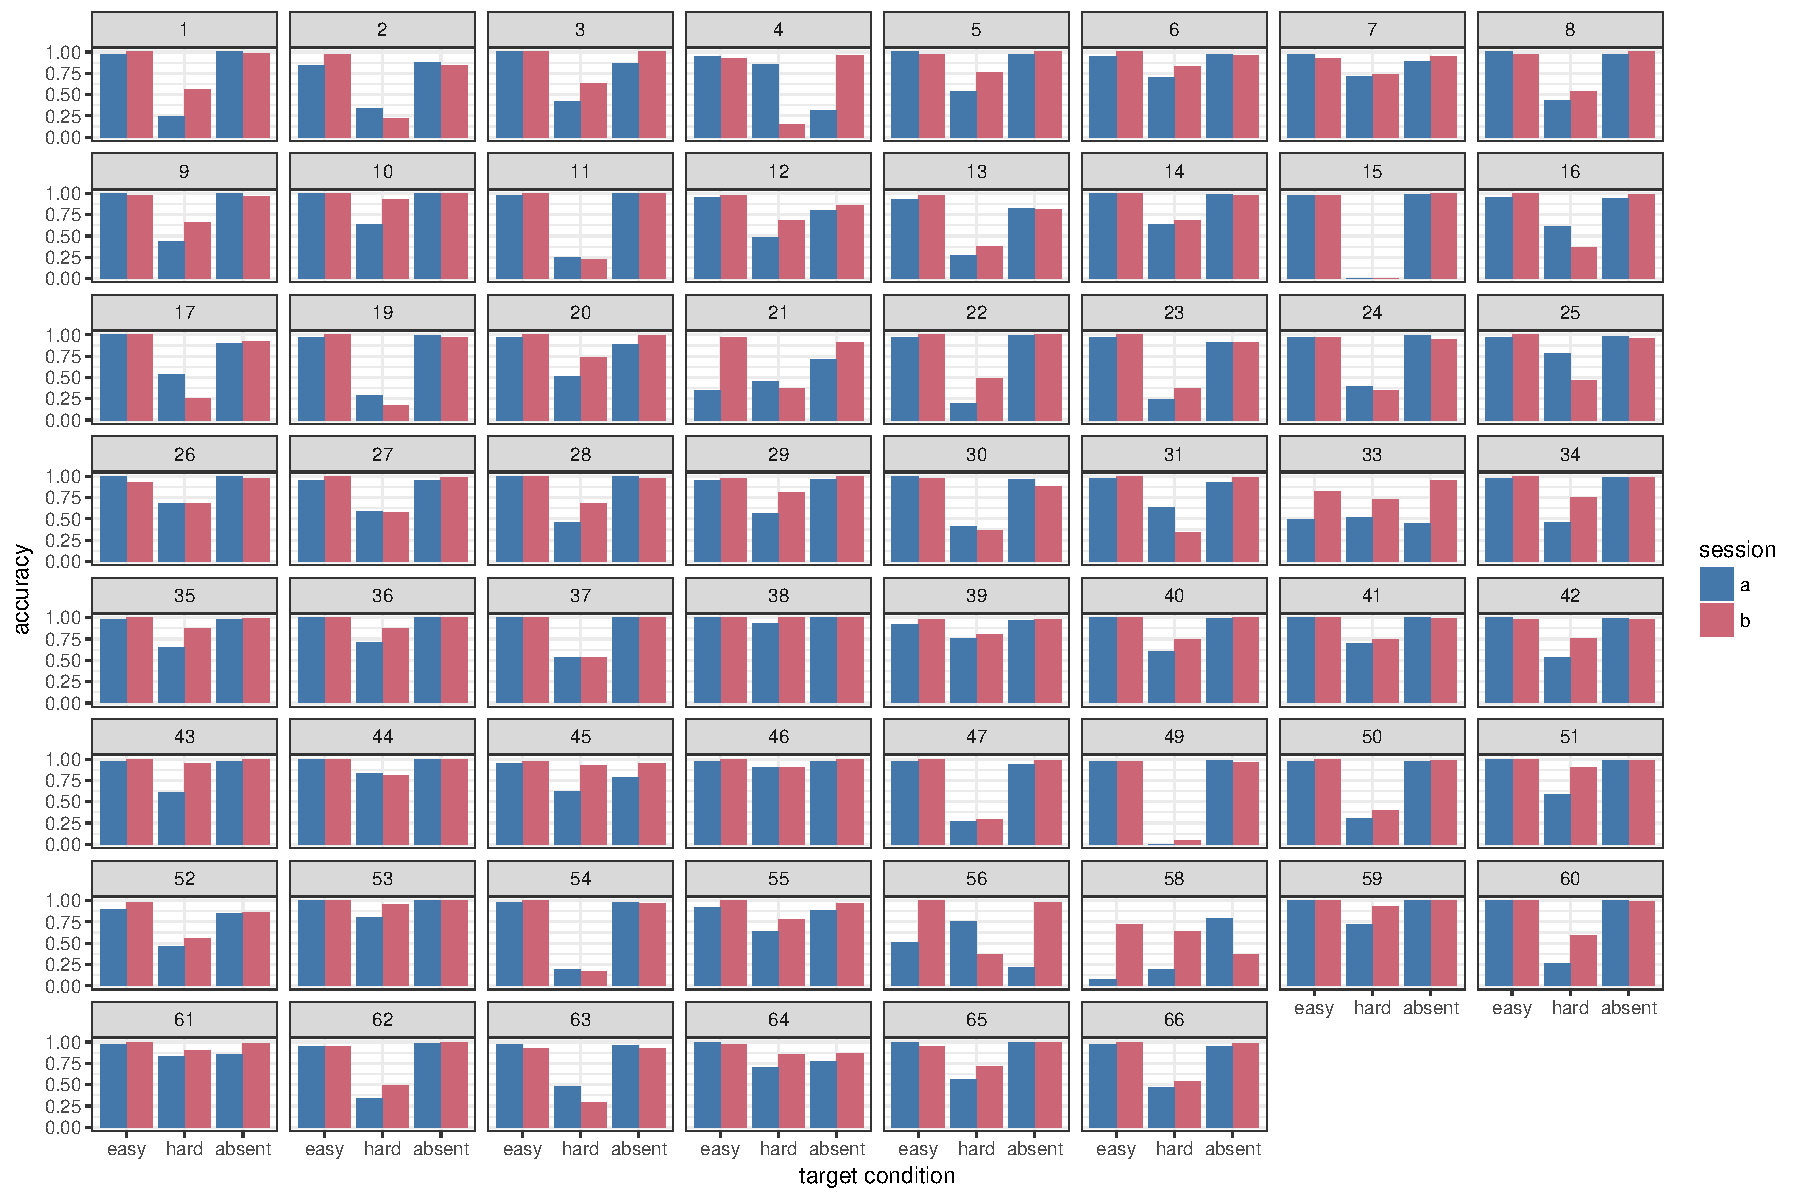
\includegraphics[width=14cm]{../Scripts/lineseg/scratch/acc_by_session_by_person.pdf}
\caption{Accuracy data for each participant for the split-half paradigm.}
\label{fig:splithalf_acc_all}
\end{figure}

\subsection{Adaptive Choice}

\subsection{Foraging}

\subsection{Comparisons across paradigms}

Interestingly, it was not the same participants who had to be removed in each paradigm. This suggests that their poor performance in one paradigm is less likely to be due to low motivation. The number of participants available for each comparison between paradigms is given in Table \ref{tab:num_per_paradigm}.

\begin{table*}
\centering
\small
\begin{tabular}{cc|c}
 		&				& Number of participants\\
 		\hline
Split-half & Adaptive Choice & \\
Split-half & Foraging & \\
Adaptive Choice & Adaptive Choice & \\


\end{tabular}

\caption{Number of participants available for each comparison}
\label{tab:num_per_paradigm}
\end{table*}







\end{document}


